\documentclass[tikz,border=10pt]{standalone}
\usepackage[T1]{fontenc}
\usepackage{amssymb}
\usetikzlibrary{positioning,arrows.meta,calc,fit,backgrounds}
\renewcommand{\familydefault}{\sfdefault}

% Okabe-Ito, matching fig_repairbench_pipeline.tex
\definecolor{cAsk}{RGB}{70,70,70}
\definecolor{cTierS}{RGB}{230,159,0}
\definecolor{cTierF}{RGB}{0,114,178}

\begin{document}
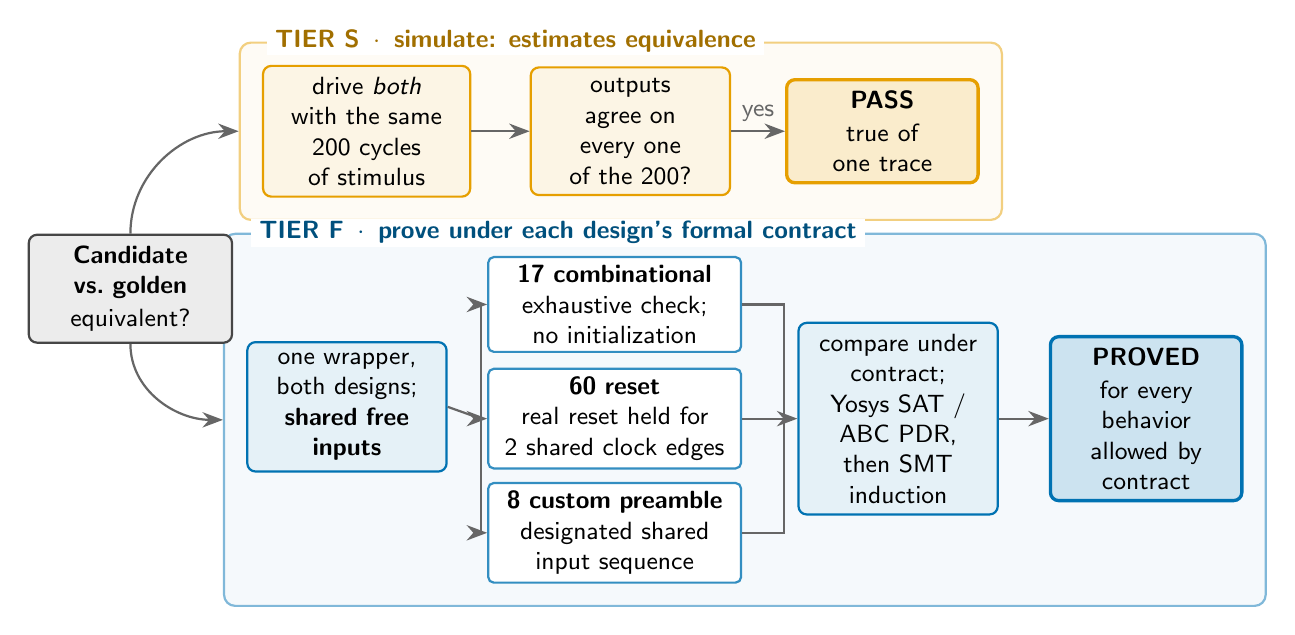
\begin{tikzpicture}[
  font=\small,
  box/.style 2 args={rounded corners=3pt, draw=#1, fill=#1!10, thick,
    align=center, inner sep=4pt, text width=#2},
  result/.style 2 args={rounded corners=3pt, draw=#1, fill=#1!20, very thick,
    align=center, inner sep=4pt, text width=#2, font=\small\bfseries},
  contract/.style={rounded corners=2pt, draw=cTierF!80, fill=white, thick,
    align=center, inner sep=3pt, text width=3.0cm, font=\small},
  lbl/.style={font=\small, text=black!60, align=center},
  arr/.style={-{Stealth[length=2.6mm]}, thick, black!60},
]

% Shared question
\node[box={cAsk}{2.3cm}] (ask) at (0,0)
  {\textbf{Candidate vs.\ golden}\\[1pt] equivalent?};

% Tier S lane
\node[box={cTierS}{2.35cm}] (s1) at (3.0,2.0)
  {drive \emph{both} with the same\\ 200 cycles of stimulus};
\node[box={cTierS}{2.25cm}] (s2) at (6.35,2.0)
  {outputs agree on\\ every one of the 200?};
\node[result={cTierS}{2.15cm}] (spass) at (9.55,2.0)
  {PASS\\[1pt] \normalfont true of one trace};

% Tier F lane
\node[box={cTierF}{2.25cm}] (f1) at (2.75,-1.5)
  {one wrapper, both designs;\\ \textbf{shared free inputs}};
\node[contract] (fcomb) at (6.15,-0.20)
  {\textbf{17 combinational}\\ exhaustive check;\\ no initialization};
\node[contract] (freset) at (6.15,-1.65)
  {\textbf{60 reset}\\ real reset held for\\ 2 shared clock edges};
\node[contract] (fpreamble) at (6.15,-3.10)
  {\textbf{8 custom preamble}\\ designated shared\\ input sequence};
\node[box={cTierF}{2.25cm}] (fsolve) at (9.75,-1.65)
  {compare under contract;\\ Yosys SAT / ABC PDR,\\ then SMT induction};
\node[result={cTierF}{2.15cm}] (fpass) at (12.9,-1.65)
  {PROVED\\[1pt] \normalfont for every behavior\\ allowed by contract};

% Lane backgrounds and labels
\begin{scope}[on background layer]
  \node[fit=(s1)(spass), draw=cTierS!50, rounded corners=4pt, inner sep=8pt,
        fill=cTierS!4, thick] (lanes) {};
  \node[fit=(f1)(fcomb)(fpreamble)(fsolve)(fpass), draw=cTierF!50,
        rounded corners=4pt, inner sep=8pt,
        fill=cTierF!4, thick] (lanef) {};
\end{scope}
\node[anchor=west, font=\small\bfseries, text=cTierS!70!black, fill=white,
      inner xsep=3pt, inner ysep=1pt]
  at ([shift={(10pt,0)}]lanes.north west) {TIER S\, $\cdot$\, simulate: \emph{estimates} equivalence};
\node[anchor=west, font=\small\bfseries, text=cTierF!70!black, fill=white,
      inner xsep=3pt, inner ysep=1pt]
  at ([shift={(10pt,0)}]lanef.north west)
  {TIER F\, $\cdot$\, prove under each design's formal contract};

% Within-lane arrows only.
\draw[arr] (ask.north) to[out=90,in=180] (lanes.west);
\draw[arr] (ask.south) to[out=-90,in=180] (lanef.west);
\draw[arr] (s1) -- (s2);
\draw[arr] (s2) -- node[lbl,above]{yes} (spass);
\coordinate (split) at (4.45,-1.65);
\coordinate (merge) at (8.30,-1.65);
\draw[thick, black!60] (f1.east) -- (split);
\draw[arr] (split) |- (fcomb.west);
\draw[arr] (split) -- (freset.west);
\draw[arr] (split) |- (fpreamble.west);
\draw[thick, black!60] (fcomb.east) -| (merge);
\draw[thick, black!60] (freset.east) -- (merge);
\draw[thick, black!60] (fpreamble.east) -| (merge);
\draw[arr] (merge) -- (fsolve.west);
\draw[arr] (fsolve) -- (fpass);

\end{tikzpicture}
\end{document}
